% Options for packages loaded elsewhere
\PassOptionsToPackage{unicode}{hyperref}
\PassOptionsToPackage{hyphens}{url}
%
\documentclass[
]{article}
\usepackage{amsmath,amssymb}
\usepackage{iftex}
\ifPDFTeX
  \usepackage[T1]{fontenc}
  \usepackage[utf8]{inputenc}
  \usepackage{textcomp} % provide euro and other symbols
\else % if luatex or xetex
  \usepackage{unicode-math} % this also loads fontspec
  \defaultfontfeatures{Scale=MatchLowercase}
  \defaultfontfeatures[\rmfamily]{Ligatures=TeX,Scale=1}
\fi
\usepackage{lmodern}
\ifPDFTeX\else
  % xetex/luatex font selection
\fi
% Use upquote if available, for straight quotes in verbatim environments
\IfFileExists{upquote.sty}{\usepackage{upquote}}{}
\IfFileExists{microtype.sty}{% use microtype if available
  \usepackage[]{microtype}
  \UseMicrotypeSet[protrusion]{basicmath} % disable protrusion for tt fonts
}{}
\makeatletter
\@ifundefined{KOMAClassName}{% if non-KOMA class
  \IfFileExists{parskip.sty}{%
    \usepackage{parskip}
  }{% else
    \setlength{\parindent}{0pt}
    \setlength{\parskip}{6pt plus 2pt minus 1pt}}
}{% if KOMA class
  \KOMAoptions{parskip=half}}
\makeatother
\usepackage{xcolor}
\usepackage[margin=1in]{geometry}
\usepackage{color}
\usepackage{fancyvrb}
\newcommand{\VerbBar}{|}
\newcommand{\VERB}{\Verb[commandchars=\\\{\}]}
\DefineVerbatimEnvironment{Highlighting}{Verbatim}{commandchars=\\\{\}}
% Add ',fontsize=\small' for more characters per line
\usepackage{framed}
\definecolor{shadecolor}{RGB}{248,248,248}
\newenvironment{Shaded}{\begin{snugshade}}{\end{snugshade}}
\newcommand{\AlertTok}[1]{\textcolor[rgb]{0.94,0.16,0.16}{#1}}
\newcommand{\AnnotationTok}[1]{\textcolor[rgb]{0.56,0.35,0.01}{\textbf{\textit{#1}}}}
\newcommand{\AttributeTok}[1]{\textcolor[rgb]{0.13,0.29,0.53}{#1}}
\newcommand{\BaseNTok}[1]{\textcolor[rgb]{0.00,0.00,0.81}{#1}}
\newcommand{\BuiltInTok}[1]{#1}
\newcommand{\CharTok}[1]{\textcolor[rgb]{0.31,0.60,0.02}{#1}}
\newcommand{\CommentTok}[1]{\textcolor[rgb]{0.56,0.35,0.01}{\textit{#1}}}
\newcommand{\CommentVarTok}[1]{\textcolor[rgb]{0.56,0.35,0.01}{\textbf{\textit{#1}}}}
\newcommand{\ConstantTok}[1]{\textcolor[rgb]{0.56,0.35,0.01}{#1}}
\newcommand{\ControlFlowTok}[1]{\textcolor[rgb]{0.13,0.29,0.53}{\textbf{#1}}}
\newcommand{\DataTypeTok}[1]{\textcolor[rgb]{0.13,0.29,0.53}{#1}}
\newcommand{\DecValTok}[1]{\textcolor[rgb]{0.00,0.00,0.81}{#1}}
\newcommand{\DocumentationTok}[1]{\textcolor[rgb]{0.56,0.35,0.01}{\textbf{\textit{#1}}}}
\newcommand{\ErrorTok}[1]{\textcolor[rgb]{0.64,0.00,0.00}{\textbf{#1}}}
\newcommand{\ExtensionTok}[1]{#1}
\newcommand{\FloatTok}[1]{\textcolor[rgb]{0.00,0.00,0.81}{#1}}
\newcommand{\FunctionTok}[1]{\textcolor[rgb]{0.13,0.29,0.53}{\textbf{#1}}}
\newcommand{\ImportTok}[1]{#1}
\newcommand{\InformationTok}[1]{\textcolor[rgb]{0.56,0.35,0.01}{\textbf{\textit{#1}}}}
\newcommand{\KeywordTok}[1]{\textcolor[rgb]{0.13,0.29,0.53}{\textbf{#1}}}
\newcommand{\NormalTok}[1]{#1}
\newcommand{\OperatorTok}[1]{\textcolor[rgb]{0.81,0.36,0.00}{\textbf{#1}}}
\newcommand{\OtherTok}[1]{\textcolor[rgb]{0.56,0.35,0.01}{#1}}
\newcommand{\PreprocessorTok}[1]{\textcolor[rgb]{0.56,0.35,0.01}{\textit{#1}}}
\newcommand{\RegionMarkerTok}[1]{#1}
\newcommand{\SpecialCharTok}[1]{\textcolor[rgb]{0.81,0.36,0.00}{\textbf{#1}}}
\newcommand{\SpecialStringTok}[1]{\textcolor[rgb]{0.31,0.60,0.02}{#1}}
\newcommand{\StringTok}[1]{\textcolor[rgb]{0.31,0.60,0.02}{#1}}
\newcommand{\VariableTok}[1]{\textcolor[rgb]{0.00,0.00,0.00}{#1}}
\newcommand{\VerbatimStringTok}[1]{\textcolor[rgb]{0.31,0.60,0.02}{#1}}
\newcommand{\WarningTok}[1]{\textcolor[rgb]{0.56,0.35,0.01}{\textbf{\textit{#1}}}}
\usepackage{graphicx}
\makeatletter
\def\maxwidth{\ifdim\Gin@nat@width>\linewidth\linewidth\else\Gin@nat@width\fi}
\def\maxheight{\ifdim\Gin@nat@height>\textheight\textheight\else\Gin@nat@height\fi}
\makeatother
% Scale images if necessary, so that they will not overflow the page
% margins by default, and it is still possible to overwrite the defaults
% using explicit options in \includegraphics[width, height, ...]{}
\setkeys{Gin}{width=\maxwidth,height=\maxheight,keepaspectratio}
% Set default figure placement to htbp
\makeatletter
\def\fps@figure{htbp}
\makeatother
\setlength{\emergencystretch}{3em} % prevent overfull lines
\providecommand{\tightlist}{%
  \setlength{\itemsep}{0pt}\setlength{\parskip}{0pt}}
\setcounter{secnumdepth}{-\maxdimen} % remove section numbering
\ifLuaTeX
  \usepackage{selnolig}  % disable illegal ligatures
\fi
\usepackage{bookmark}
\IfFileExists{xurl.sty}{\usepackage{xurl}}{} % add URL line breaks if available
\urlstyle{same}
\hypersetup{
  pdftitle={Q2 SLR: station\_precipitation},
  hidelinks,
  pdfcreator={LaTeX via pandoc}}

\title{Q2 SLR: station\_precipitation}
\author{}
\date{\vspace{-2.5em}2024-12-06}

\begin{document}
\maketitle

\section{Question 2}\label{question-2}

Exam Question:

In regional precipitation-frequency analysis, predicting the mean annual
maximum precipitation at study sites using seasonal total precipitation
as a predictor is a common approach. This allows researchers to estimate
mean annual maximum precipitation in locations where seasonal total
precipitation can be estimated.

PRISM climate normals provide spatially continuous maps of long-term
averages for meteorological variables such as temperature and
precipitation. Using PRISM as the basis for regression analysis enables
predictions to be made almost anywhere. For this exercise, you will work
with two variables from the dataset: seasonal total precipitation
(predictor) and mean annual maximum precipitation (response).

\begin{itemize}
\tightlist
\item
  Perform a linear regression to evaluate whether seasonal total
  precipitation is a significant predictor of mean annual maximum
  precipitation.
\item
  Evaluate the model's assumptions, including normality of residuals and
  homoscedasticity. If any assumptions appear to be violated, explore
  possible reasons for the violations and suggest ways to address them.
\item
  Investigate whether any influential observations might be affecting
  the model fit by calculating and interpreting diagnostic metrics
  (e.g., Cook's Distance). Use these findings to propose or implement
  improvements to the model.
\item
  Summarize your analysis in a clear, concise paragraph, including your
  regression results, assumption checks, and any modifications made to
  the model.
\end{itemize}

\begin{Shaded}
\begin{Highlighting}[]
\NormalTok{data }\OtherTok{\textless{}{-}} \FunctionTok{read.csv}\NormalTok{(}\StringTok{\textquotesingle{}Q2{-}SLR{-}station precipitation.csv\textquotesingle{}}\NormalTok{)}
\FunctionTok{head}\NormalTok{(data)}
\end{Highlighting}
\end{Shaded}

\begin{verbatim}
##          name   n      l_1        t       t_3       t_4 Latitude Longitude
## 1 US1ORBN0013  85 4.949470 0.145362  0.149513  0.164376  44.6383 -123.5772
## 2 US1ORDG0044  44 5.656320 0.158076 -0.011484  0.028511  43.6918 -124.1246
## 3 US1ORLA0088  66 5.326953 0.130497  0.132726  0.121872  43.9087 -124.0884
## 4 US1ORLC0002  23 5.646357 0.198023  0.308209  0.142237  44.6210 -123.9370
## 5 US1ORLC0013 103 4.788742 0.182743  0.166362  0.116272  44.6773 -124.0592
## 6 US1ORTL0004  17 6.838586 0.181588 -0.161657 -0.010757  45.7235 -123.9391
##          Station_Na pm_wnt_ppt pm_wnt_tmp pm_elev  DISTCOAST RFA_Region
## 1      BLODGETT 1 N    1007.43     5.5800     252 33.7814441      ABCD1
## 2  REEDSPORT 0.8 SW    1115.48     8.0750      20  5.0414342      ABCD1
## 3    FLORENCE 5.4 S    1057.24     7.8875      43  5.6614377      ABCD1
## 4      TOLEDO 0.2 W    1009.03     7.7275      53  5.8014491      ABCD1
## 5     NEWPORT 4.2 N    1025.60     8.2275      46  0.1890756      ABCD1
## 6 MANZANITA 0.5 NNW    1279.41     7.8125      14  0.5914717      ABCD1
##   orig_reg
## 1        B
## 2        C
## 3        C
## 4        B
## 5        B
## 6        B
\end{verbatim}

\subsection{Set up regression}\label{set-up-regression}

\begin{Shaded}
\begin{Highlighting}[]
\NormalTok{mod1 }\OtherTok{\textless{}{-}} \FunctionTok{lm}\NormalTok{(l\_1 }\SpecialCharTok{\textasciitilde{}}\NormalTok{ pm\_wnt\_ppt, data)}
\FunctionTok{summary}\NormalTok{(mod1)}
\end{Highlighting}
\end{Shaded}

\begin{verbatim}
## 
## Call:
## lm(formula = l_1 ~ pm_wnt_ppt, data = data)
## 
## Residuals:
##     Min      1Q  Median      3Q     Max 
## -3.5414 -0.3310  0.0015  0.2888  2.0889 
## 
## Coefficients:
##               Estimate Std. Error t value            Pr(>|t|)    
## (Intercept) 0.73793839 0.08262761   8.931 <0.0000000000000002 ***
## pm_wnt_ppt  0.00435654 0.00008177  53.275 <0.0000000000000002 ***
## ---
## Signif. codes:  0 '***' 0.001 '**' 0.01 '*' 0.05 '.' 0.1 ' ' 1
## 
## Residual standard error: 0.5558 on 293 degrees of freedom
## Multiple R-squared:  0.9064, Adjusted R-squared:  0.9061 
## F-statistic:  2838 on 1 and 293 DF,  p-value: < 0.00000000000000022
\end{verbatim}

\section{Get standardized residuals}\label{get-standardized-residuals}

\begin{Shaded}
\begin{Highlighting}[]
\NormalTok{mod1.res }\OtherTok{\textless{}{-}} \FunctionTok{rstandard}\NormalTok{(mod1)}
\FunctionTok{shapiro.test}\NormalTok{(mod1.res)}
\end{Highlighting}
\end{Shaded}

\begin{verbatim}
## 
##  Shapiro-Wilk normality test
## 
## data:  mod1.res
## W = 0.91601, p-value = 0.000000000008453
\end{verbatim}

\section{The Breusch-Pagan test to assess
homoscedasticity}\label{the-breusch-pagan-test-to-assess-homoscedasticity}

\begin{Shaded}
\begin{Highlighting}[]
\FunctionTok{ncvTest}\NormalTok{(mod1)}
\end{Highlighting}
\end{Shaded}

\begin{verbatim}
## Non-constant Variance Score Test 
## Variance formula: ~ fitted.values 
## Chisquare = 47.57819, Df = 1, p = 0.0000000000052853
\end{verbatim}

\#Cooks D

\begin{Shaded}
\begin{Highlighting}[]
\FunctionTok{ggplot}\NormalTok{(}\FunctionTok{as\_tibble}\NormalTok{(}\FunctionTok{cooks.distance}\NormalTok{(mod1)), }\FunctionTok{aes}\NormalTok{(value)) }\SpecialCharTok{+} \FunctionTok{geom\_boxplot}\NormalTok{()}
\end{Highlighting}
\end{Shaded}

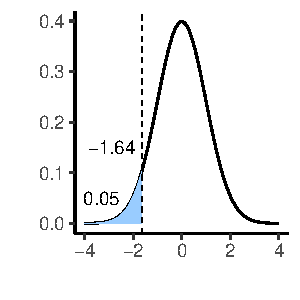
\includegraphics{Q2-SLR-station-precipitation_files/figure-latex/unnamed-chunk-3-1.pdf}

\begin{Shaded}
\begin{Highlighting}[]
\FunctionTok{plot}\NormalTok{(mod1,}\AttributeTok{which=}\DecValTok{4}\NormalTok{)}
\end{Highlighting}
\end{Shaded}

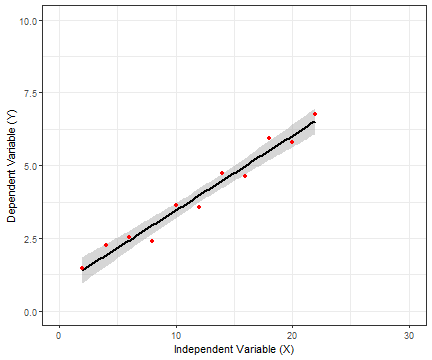
\includegraphics{Q2-SLR-station-precipitation_files/figure-latex/unnamed-chunk-3-2.pdf}

\section{Make plot of beaver dams and surface
water}\label{make-plot-of-beaver-dams-and-surface-water}

\begin{Shaded}
\begin{Highlighting}[]
\FunctionTok{plot}\NormalTok{(l\_1 }\SpecialCharTok{\textasciitilde{}}\NormalTok{ pm\_wnt\_ppt, data, }
     \AttributeTok{pch =} \DecValTok{19}\NormalTok{, }
     \AttributeTok{col =} \StringTok{"royalblue4"}\NormalTok{,}
     \AttributeTok{ylab =} \StringTok{"Surface water area (ha)"}\NormalTok{,}
     \AttributeTok{xlab =}  \StringTok{"Number of beaver dams"}\NormalTok{)}
\CommentTok{\#add regression line}
\CommentTok{\#make line width thicker}
\FunctionTok{abline}\NormalTok{(mod1, }\AttributeTok{lwd=}\DecValTok{2}\NormalTok{)}
\end{Highlighting}
\end{Shaded}

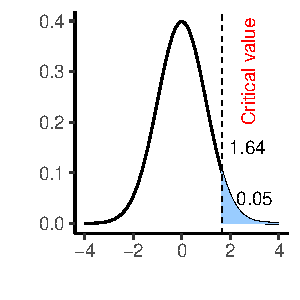
\includegraphics{Q2-SLR-station-precipitation_files/figure-latex/unnamed-chunk-4-1.pdf}

\section{}\label{section}

The linear regression model indicates that seasonal total precipitation
(pm\_wnt\_ppt) is a highly significant predictor of mean annual maximum
precipitation (p \textless{} 0.001), with an adjusted R2R2 of 0.9061,
suggesting the model explains a large portion of the variability in the
response. However, diagnostic checks reveal violations of assumptions:

\begin{itemize}
\tightlist
\item
  Residual Normality: The Shapiro-Wilk test is significant
  (W=0.916,p\textless0.001W=0.916,p\textless0.001), indicating
  non-normal residuals.
\item
  Heteroscedasticity: The non-constant variance test is significant
  (χ2=47.58,p\textless0.001χ2=47.58,p\textless0.001), showing
  heteroscedasticity.
\item
  Influential Points: Cook's Distance analysis suggests potential
  influence from observations 143, 258, and 290, which warrant further
  investigation.
\end{itemize}

These issues suggest the need for model improvements, such as addressing
outliers or transforming variables.

\section{References:}\label{references}

\end{document}
